\begin{figure}[hbt!]
    \begin{subfigure}[b]{0.5\textwidth}
        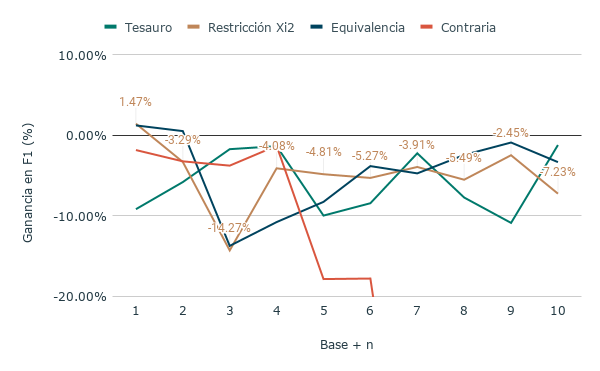
\includegraphics[width=\textwidth]{sections/figures/bi_LSTMAnox.png}
        \caption{Bi-LSTM}
    \end{subfigure}
    \hfill
    \begin{subfigure}[b]{0.5\textwidth}
        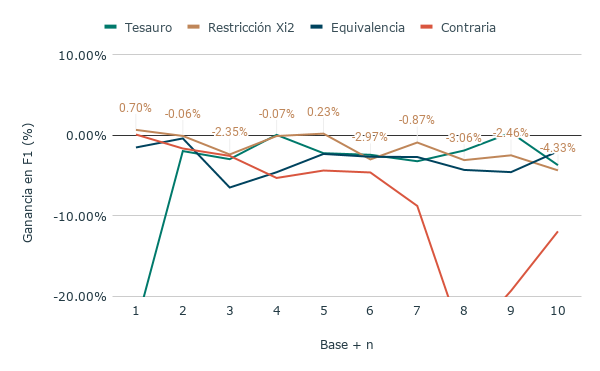
\includegraphics[width=\textwidth]{sections/figures/CNNAnox.png}
        \caption{CNN}
    \end{subfigure}
    \hfill
    
    
    \caption{Relación entre el aumento del conjunto de datos \textit{Anorexia} y la ganancia porcentual en F1.}
    \label{fig:aumento_n_anorexia}
\end{figure}